
\section{DC Buck-Boost Converter (High Ratings)}

\subsection{Open-Loop System Model (with Resistive Load)}

In the open-loop mode, a fixed duty cycle is applied to control the switching device without any feedback mechanism. Consequently, the output voltage depends solely on the input voltage, duty cycle, and circuit parameters. The output voltage follows the conventional buck--boost converter\cite{mohan2003}:

\begin{equation}
V_{out}=\frac{D\,V_{in}}{1-D}
\end{equation}

\subsubsection{Simulation Model}

\begin{figure}[H]
    \centering
    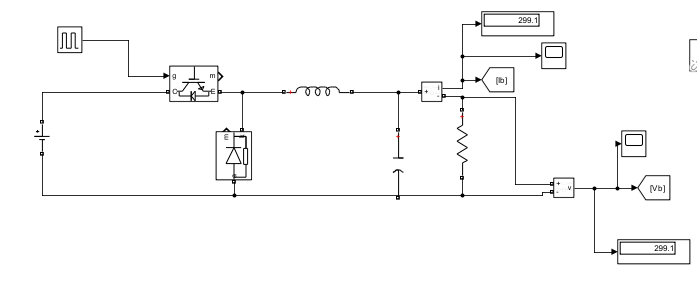
\includegraphics[width=0.85\textwidth]{Figures/2.png}
    \caption{Open-loop Two-Quadrant Chopper with Resistive Load}
    \label{fig:open_loop_resistor}
\end{figure}

\subsubsection{Results}

The converter performance was evaluated using different duty-cycle values.

\begin{itemize}
    \item Duty Cycle $D=0.5$
    \begin{figure}[H]
    \centering
    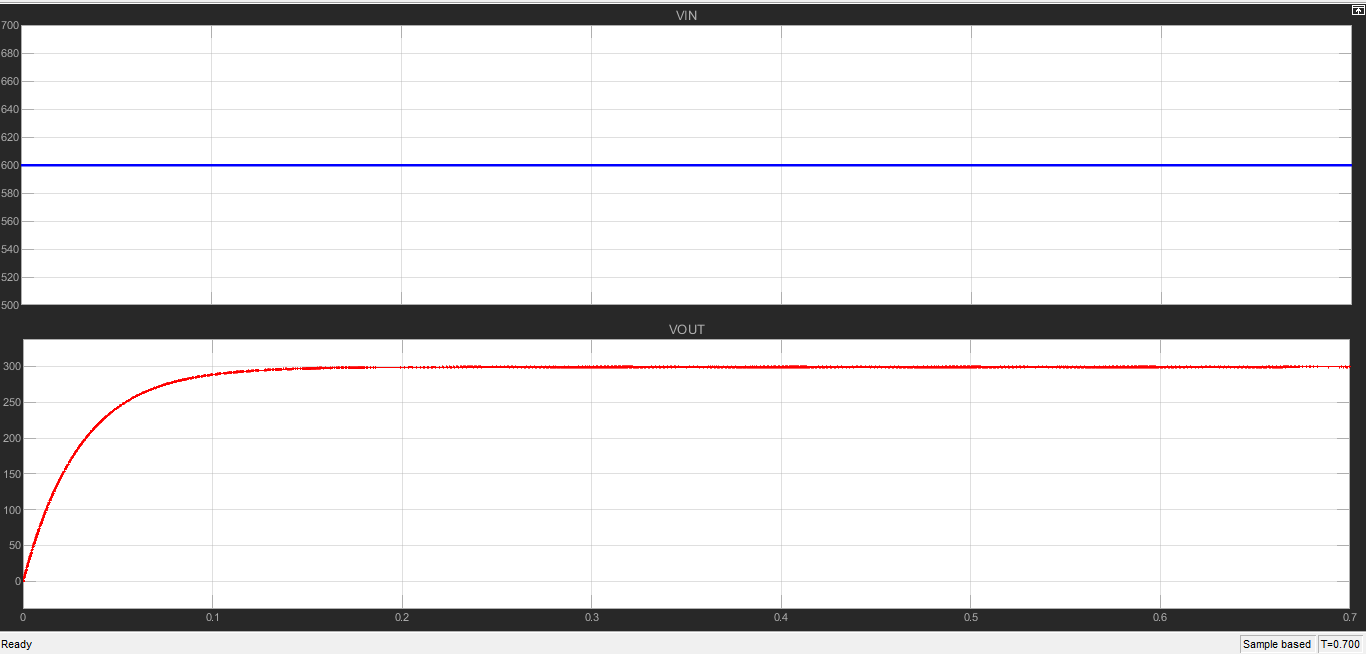
\includegraphics[width=0.85\textwidth]{Figures/0.5.png}
    \caption{Input and Output Voltage for duty cycle = 0.5}
    \label{fig:open_loop_resistor}
\end{figure}
    \item Duty Cycle $D=0.7$
    \begin{figure}[H]
    \centering
    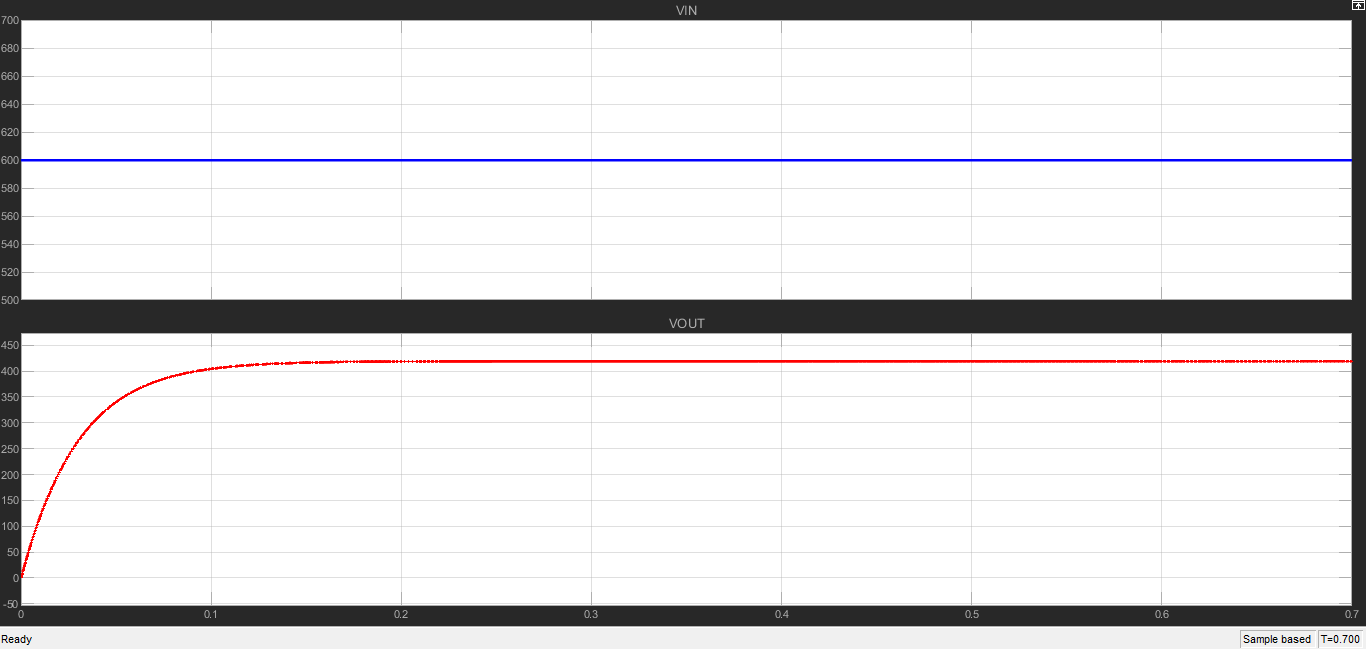
\includegraphics[width=0.85\textwidth]{Figures/0.7.png}
    \caption{Input and Output Voltage for duty cycle = 0.7}
    \label{fig:open_loop_resistor}
\end{figure}
    
\end{itemize}

%%%%%%%%%%%%%%%%%%%%%%%%%%%%%%%%%%%%%%%%%%%%%%%%%%%%%%%%%%

\subsection{Open-Loop System Model (Battery Modeled as an RC Load with CC--CV Control)}

In this configuration, the battery is represented by an equivalent RC circuit while the converter still operates in open-loop mode using a fixed duty cycle. The output voltage continues to follow the buck--boost converter equation:

\begin{equation}
V_{out}=\frac{D\,V_{in}}{1-D}
\end{equation}

\subsubsection{Simulation Model}

\begin{figure}[H]
    \centering
    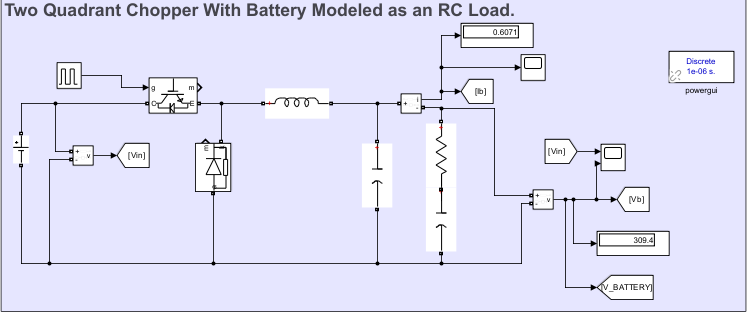
\includegraphics[width=0.85\textwidth]{Figures/3.png}
    \caption{Open-loop Two-Quadrant Chopper with RC Battery Model}
    \label{fig:open_loop_rc}
\end{figure}
\newpage
\subsubsection{Results}

The converter performance was evaluated using different duty-cycle values.

\begin{itemize}
    \item Duty Cycle $D=0.5$
    \begin{figure}[H]
    \centering
    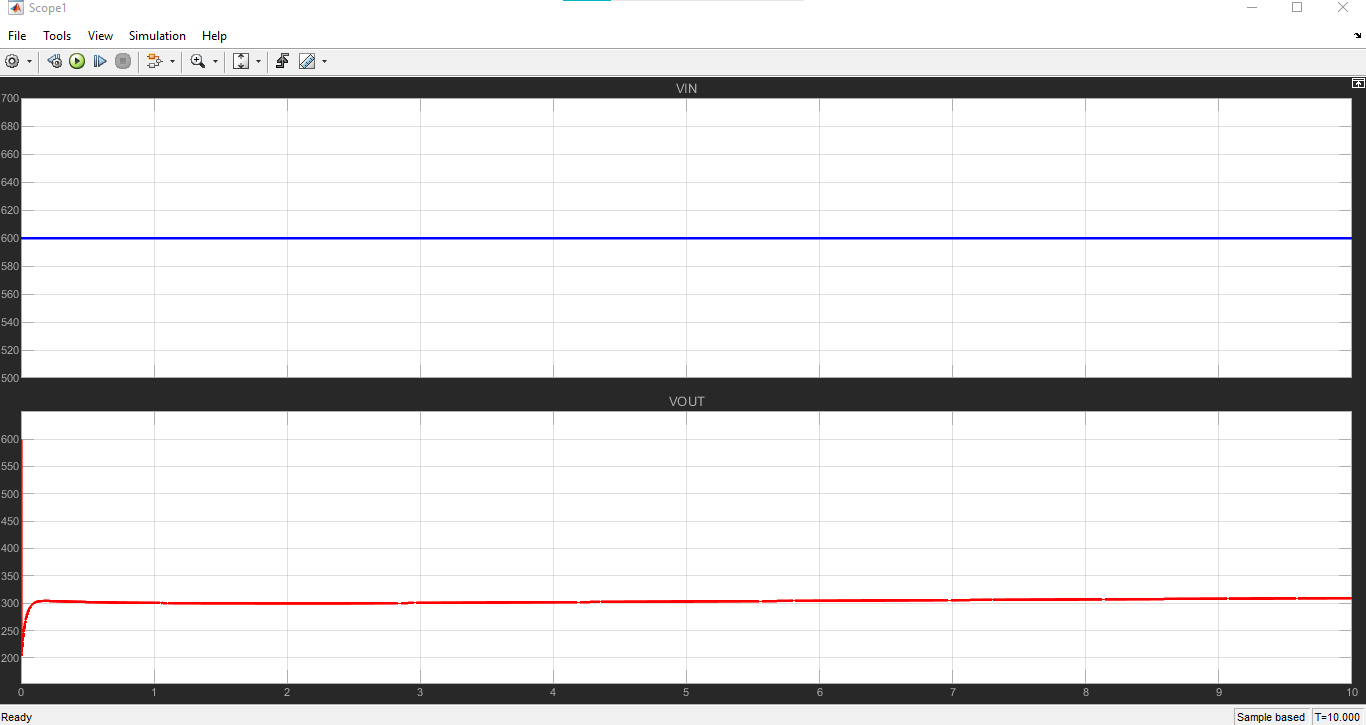
\includegraphics[width=0.85\textwidth]{Figures/2Q/D50 RC.png}
    \caption{Input and Output Voltage for duty cycle = 0.5}
    \label{fig:open_loop_resistor}
\end{figure}
    \item Duty Cycle $D=0.7$
    \begin{figure}[H]
    \centering
    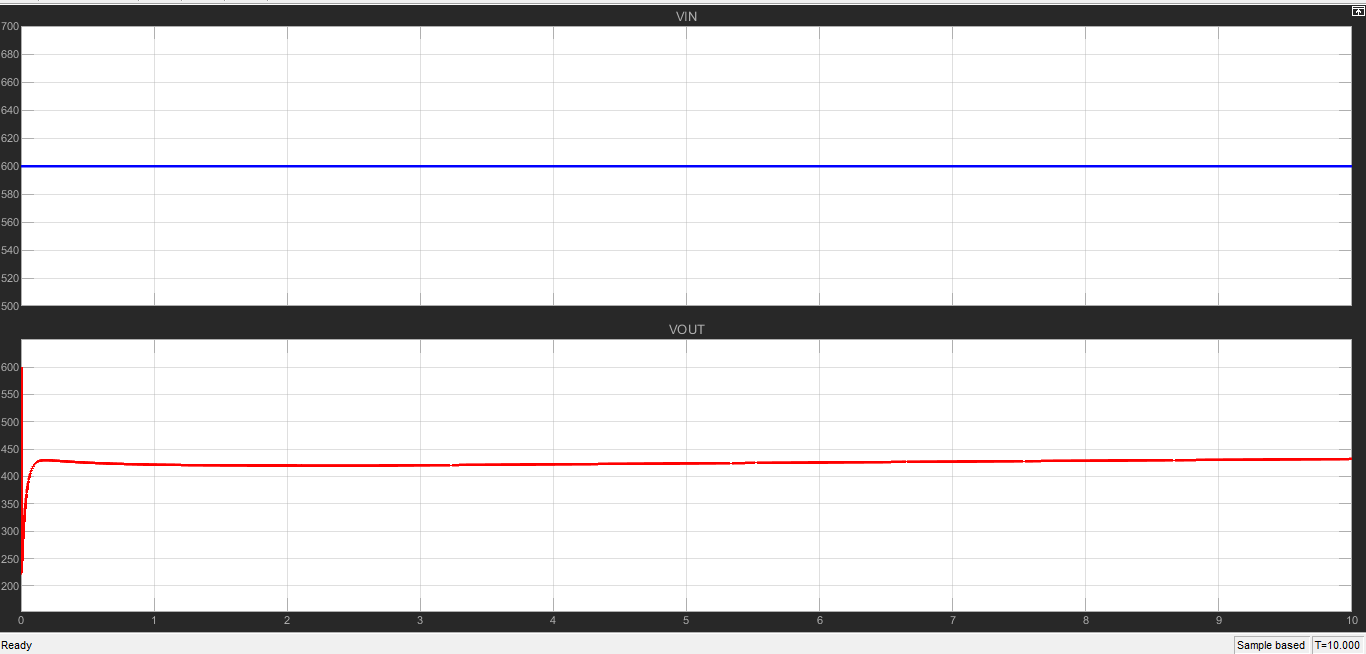
\includegraphics[width=0.85\textwidth]{Figures/D70RC.png}
    \caption{Input and Output Voltage for duty cycle = 0.7}
    \label{fig:open_loop_resistor}
\end{figure}
    
\end{itemize}



%%%%%%%%%%%%%%%%%%%%%%%%%%%%%%%%%%%%%%%%%%%%%%%%%%%%%%%%%%

\subsection{Closed-Loop System (Battery Modeled as an RC Load with CC--CV Control)}

To represent the battery charging process more realistically, the ideal battery was replaced with an equivalent electrical model consisting of a resistor and capacitor connected in series (RC model). The capacitor represents the battery storage capacity, whereas the resistor models the internal resistance.
\newpage
The charging behavior is governed by the RC time constant,

\begin{equation}
\tau=RC
\end{equation}

where

\[
R=1~\Omega,\qquad C=0.5~\mathrm{F}
\]

thus,

\[
\tau=0.5~\mathrm{s}
\]

%%%%%%%%%%%%%%%%%%%%%%%%%%%%%%%%%%%%%%%%%%%%%%%%%%%%%%%%%%

\subsubsection{Constant Current (CC) Stage}

Initially, the battery is charged using a constant current regulated by a PI current controller. During this stage, the battery voltage increases gradually according to the RC charging characteristics.

\begin{figure}[H]
    \centering
    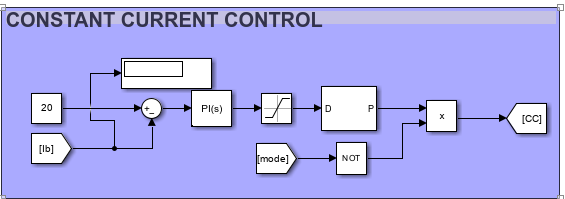
\includegraphics[width=0.8\textwidth]{Figures/cc.png}
    \caption{Constant Current Control}
    \label{fig:cc_control}
\end{figure}

%%%%%%%%%%%%%%%%%%%%%%%%%%%%%%%%%%%%%%%%%%%%%%%%%%%%%%%%%%

\subsubsection{Constant Voltage (CV) Stage}

Once the battery voltage reaches the predefined limit of approximately $570~\mathrm{V}$, the control system automatically switches to the voltage PI controller. During this stage, the battery voltage is maintained at the reference value while the charging current gradually decreases toward zero, indicating the completion of the charging process.

\begin{figure}[H]
    \centering
    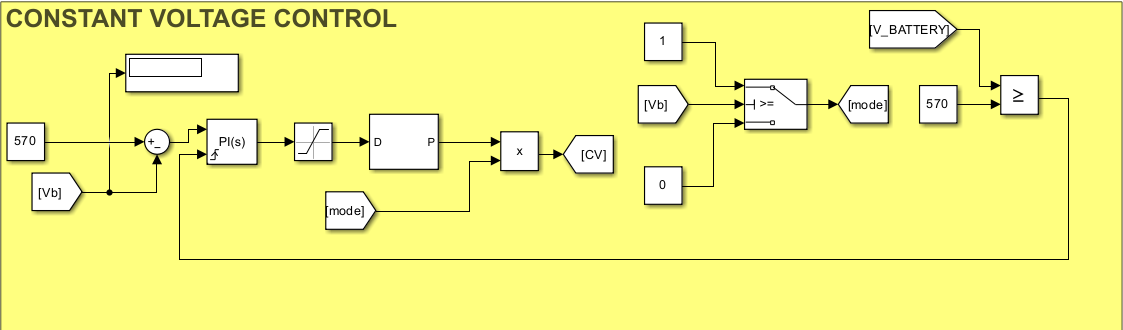
\includegraphics[width=0.8\textwidth]{Figures/cv.png}
    \caption{Constant Voltage Control}
    \label{fig:cv_control}
\end{figure}

%%%%%%%%%%%%%%%%%%%%%%%%%%%%%%%%%%%%%%%%%%%%%%%%%%%%%%%%%%

\subsubsection{Results}

\paragraph{CC--CV Charging Profile}

\begin{figure}[H]
    \centering
    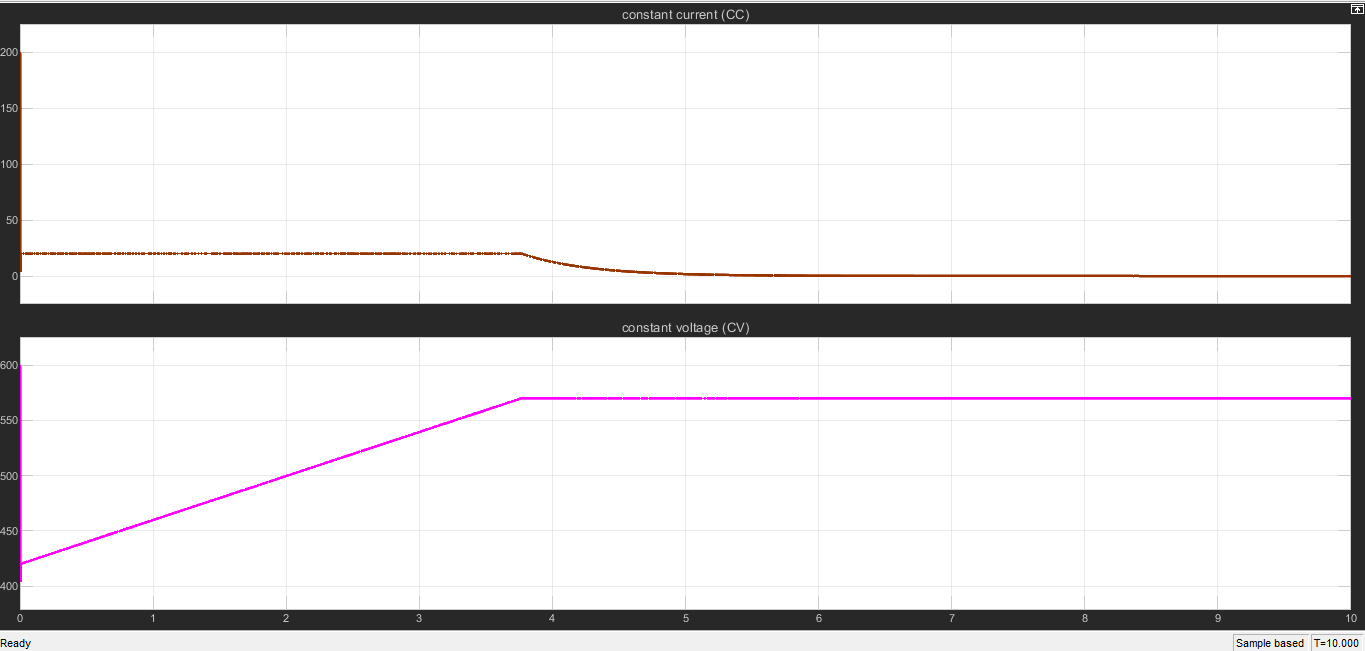
\includegraphics[width=0.85\textwidth]{Figures/cc-cv.png}
    \caption{CC--CV Charging Profile of the Energy Storage System}
    \label{fig:cc_cv_profile}
\end{figure}

The charging profile illustrates the two-stage charging strategy. During the Constant Current (CC) stage, the controller maintains a fixed charging current to maximize charging efficiency. Once the battery voltage reaches the safety threshold, the controller transitions smoothly to the Constant Voltage (CV) stage. During this phase, the charging current decreases gradually while maintaining the battery voltage at its reference value, ensuring safe and reliable battery charging.

%%%%%%%%%%%%%%%%%%%%%%%%%%%%%%%%%%%%%%%%%%%%%%%%%%%%%%%%%%

\paragraph{Voltage Regulation}

\begin{figure}[H]
    \centering
    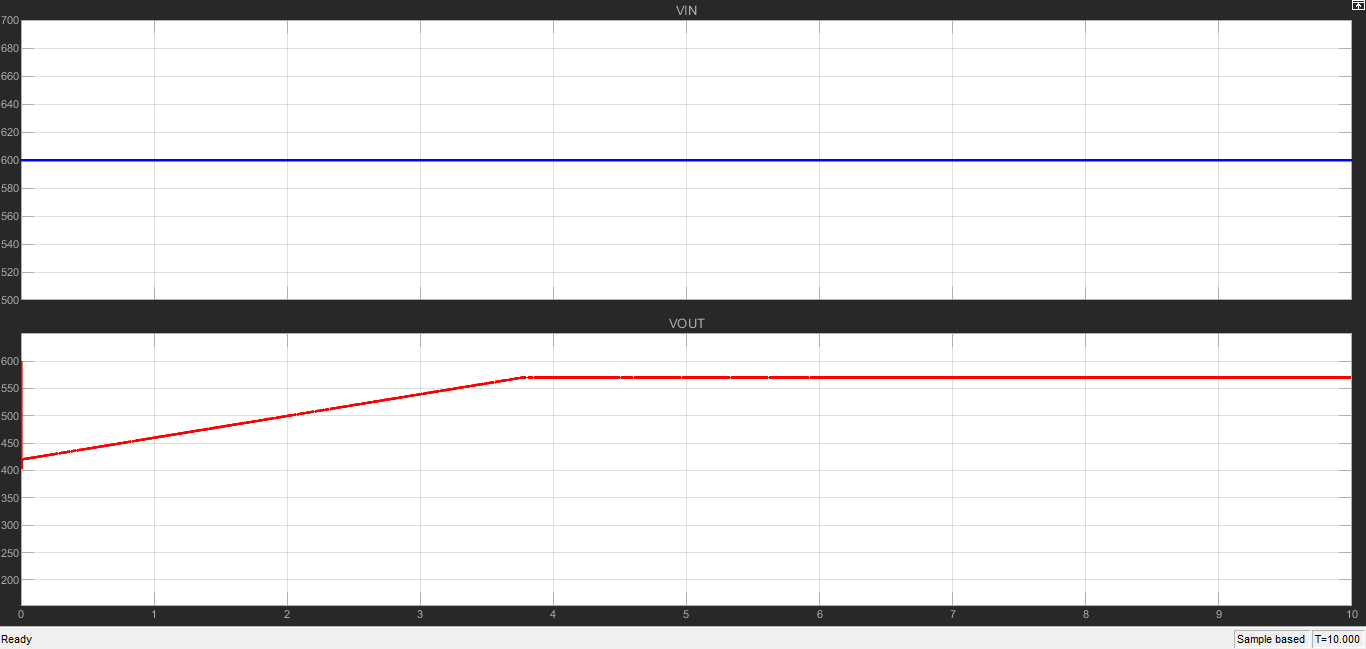
\includegraphics[width=0.85\textwidth]{Figures/v.png}
    \caption{Voltage Conversion from the DC Bus to the Energy Storage System}
    \label{fig:voltage_regulation}
\end{figure}

The waveform demonstrates the voltage conversion from the 600 V DC bus to the regulated battery charging voltage of approximately 570 V. The controller accurately maintains this voltage level during the Constant Voltage stage, ensuring that the battery is charged safely while preventing over-voltage conditions.